% The antipodal cross: the four embeddings as two antipodal pairs on the axes.
% Compile from figures/ (the fonts resolve relative to the cwd): lualatex naive_cross.tex,
% then pdftoppm -png -r 200 and autocrop to naive_cross.png (see ../reproduce.sh).
\documentclass{article}
\usepackage[a4paper, margin=1cm]{geometry}
\pagestyle{empty}
\usepackage{fontspec}
\usepackage{xcolor}
\usepackage{amsmath}
\usepackage{tikz}
\setmainfont{Poppins}[
  Path = fonts/Poppins/,
  Extension = .ttf,
  UprightFont = *-Regular,
  BoldFont = *-Bold,
  ItalicFont = *-Italic,
  BoldItalicFont = *-BoldItalic
]
\definecolor{pivotalBlue}{HTML}{3A82B5}
\definecolor{pivotalTaupe}{HTML}{818089}
\tikzset{
  feat/.style={-stealth, line width=2.4pt, pivotalBlue},
  axis/.style={-stealth, line width=1pt, pivotalTaupe!70},
  lbl/.style={font=\fontsize{17}{20}\selectfont},
}
\begin{document}
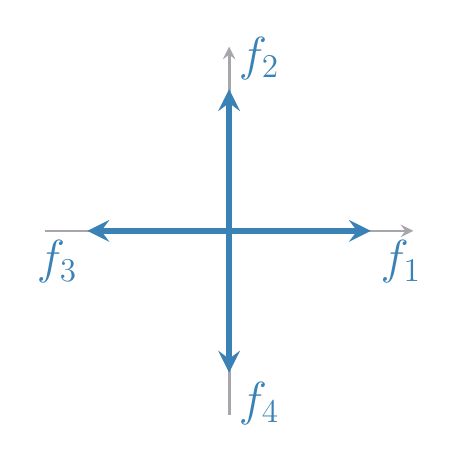
\begin{tikzpicture}[scale=1.8]
  \draw[axis] (-1.3,0) -- (1.3,0);
  \draw[axis] (0,-1.3) -- (0,1.3);
  \foreach \a in {0, 90, 180, 270} { \draw[feat] (0,0) -- (\a:1); }
  \node[pivotalBlue, below right, lbl] at (1,0)  {$f_1$};
  \node[pivotalBlue, above right, lbl] at (0,1)  {$f_2$};
  \node[pivotalBlue, below left,  lbl] at (-1,0) {$f_3$};
  \node[pivotalBlue, below right, lbl] at (0,-1) {$f_4$};
\end{tikzpicture}
\end{document}
